\problemname{H: Kabobs}
\balloon{5f7a47}

\noindent
Anna wants to open a marvelous restaurant, ``Candy Mountain'', serving only
candy \emph{kabobs}: sticks on which one puts various pieces of food, to be
eaten from the tip to the base.

Like other kabob enthusiasts,
when Anna eats a pattern of consecutive types of food in a kabob, she expects
to eat another pattern later in the kabob.
For instance, once she eats a
piece of apple immediately followed by a piece of banana, she expects to have a
leaf of mint immediately followed by chocolate in the remaining part of the
kabob.
She is
happy if she finds this mint-chocolate pattern anywhere in
the remaining kabob pieces.

Here is a kabob
 that Anna likes:
\[\texttt{Apple-Banana-Watermelon-Plum-Watermelon-Plum-Watermelon-Mint-Chocolate}\]
or, graphically:
\begin{center}
\includegraphics[width=\textwidth]{kabob.pdf}
\end{center}

Anna has written down her perfect set of kabob patterns for the new
restaurant, but she worries that these rules would give too many
potential kabob types.  This set of patterns is written down as a
\emph{ruleset},
where each rule is of the form ``$b$ implies $e$ afterwards'', where $b$ and
$e$ are non-empty sequences of characters, representing food pieces. A
rule of the form $b\,\texttt{>}\,e$ with $b=b_1 \ldots b_k$ and $e=e_1 \ldots e_l$
means that, if the pattern $b$ is encountered in the kabob, then the
kabob should also contain $e$ at some point after. Each $b_{i+1}$ must
immediately follow $b_i$ to trigger the rule and similarly each $e_{j+1}$
must immediately follow $e_j$ to satisfy it, but $b_k$ and $e_1$ do
not need to be consecutive.
No food piece can appear more than once in a rule (i.e.,
there is no $i,j$ such that $e_j=b_i$ and no $i\neq j$ with $b_i=b_j$ or
$e_i=e_j$) but a food piece can appear in several rules.

Note that if there are several occurrences of the word $b$ in a kabob, they all
need to be followed by an $e$. This can be a single $e$,
as long as this $e$ appears after all the $b$.

In a ruleset, rules are separated by `\texttt{|}' and are of the
form $u\,\texttt{>}\,v$ meaning that each pattern $u$ implies a pattern $v$
afterwards. $u$ and $v$ are words composed of alphanumerical characters and no
character can appear twice in a rule.
For instance, the ruleset
``\texttt{AB>X|R>A|T>B}'' describes three rules:
\begin{itemize}
\item for each \texttt{AB} there must be an \texttt{X}
  afterwards;
\item for each \texttt{R} there must be an \texttt{A} afterwards; and
\item for each \texttt{T} there must be a \texttt{B} afterwards.
\end{itemize}
Using this ruleset, the kabobs
\texttt{SBSB}, \texttt{REA}, \texttt{ABX}, \texttt{BA}, \texttt{ABXBA}, \texttt{RRA}, \texttt{TBTB}, and
\texttt{RTABX} are valid; but \texttt{RAT}, \texttt{TAB}, and
\texttt{ABXAB} are not.

Anna asks you how many kabobs of a given size are compatible with her ruleset.

\subsection*{Input}

\begin{itemize}
\item The first line contains an integer $K$, the size of all kabobs,
  followed with a space, and a
  non-empty string $S$ of alphanumerical characters (`\texttt{A}' to `\texttt{Z}',
    `\texttt{a}' to `\texttt{z}', and `\texttt{0}' to `\texttt{9}'),
  representing the elements that can be used in a kabob (no
  characters appear twice in $S$).
\item The second line contains a non-empty string $R$, which contains no spaces and represents
  a ruleset as described above. The patterns in $R$ are composed of characters from $S$ only.
\end{itemize}

\subsection*{Limits}

The input is such that $1 \leq K \leq 500$ and $3\leq |R| \leq 60$.

\subsection*{Output}

One integer: the number of kabobs of length~$K$ satisfying all
the rules in~$R$, modulo $10\,000\,000$.

% AABC, ABBC, ABCC, BABC, BBBC, BBCC, BCCC, CABC, CCCC
